Quoting @alpacaherder@ubuntu.social:
\url{https://ubuntu.social/@alpacaherder/110080506419926833} \#retoot

\begin{figure}
\centering
\pandocbounded{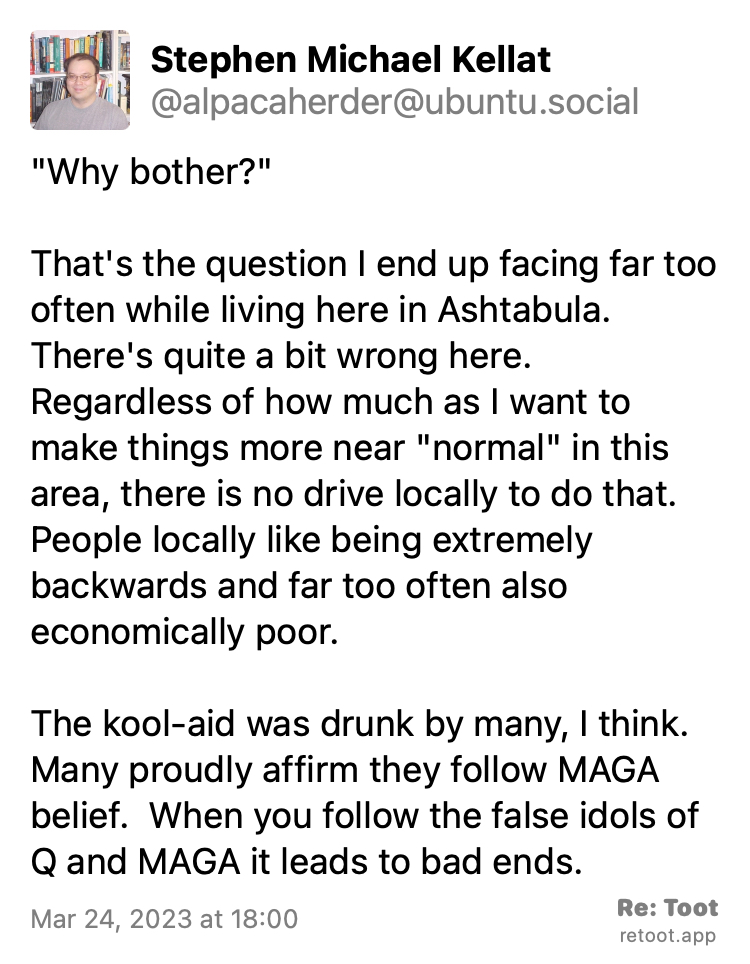
\includegraphics[keepaspectratio]{\%7B\%7Bsite.url\%7D\%7D/img/depression-brain-1.jpg}}
\caption{Post by Stephen Michael Kellat. ``\,``Why bother?'' That's the
question I end up facing far too often while living here in Ashtabula.
There's quite a bit wrong here. Regardless of how much as I want to make
things more near ``normal'' in this area, there is no drive locally to
do that. People locally like being extremely backwards and far too often
also economically poor. The kool-aid was drunk by many, I think. Many
proudly affirm they follow MAGA belief. When you follow the false idols
of Q and MAGA it leads to bad ends.'' Posted on Mar 24, 2023 at 18:00}
\end{figure}

Yeah, I do get upset at points. I gets batted about whether it is
``depression brain'' talking or if it is a reflection of the state of
the ara. For as long as I have been alive it has been a saying that you
set your clocks back twenty years when you cross the county line into
Ashtabula County. Nowadays I would say it isn't twenty but rather thirty
to forty.

The area wants to cling to glory days that are in the continually
receding past. In the county health rankings from the University of
Wisconsin, Ashtabula County is
\href{https://www.countyhealthrankings.org/explore-health-rankings/ohio/ashtabula?year=2022}{among
the very least health counties in Ohio}. Life expectancy here is lower
than not just the national average but the state average too! When you
pull up ``peer counties'' that have similar socioeconomic indicators as
well as demographic indicators the rankings site gives you choices like
these counties across the country:

\begin{itemize}
\tightlist
\item
  Cattaraugus County, New York
\item
  Cayuga County, New York
\item
  Chautauqua County, New York
\item
  Clearfield County, Pennsylvania
\item
  Clinton County, New York
\item
  Columbiana County, Ohio
\item
  Crawford County, Pennsylvania
\item
  Cullman County, Alabama
\item
  Erie County, Ohio
\item
  Fulton County, New York
\item
  Grant County, Indiana
\item
  Greene County, Tennessee
\item
  Harrison County, West Virginia
\item
  Indiana County, Pennsylvania
\item
  Kennebec County, Maine
\item
  LaSalle County, Illinois
\item
  Lawrence County, Pennsylvania
\item
  Lenawee County, Michigan
\item
  Marion County, West Virginia
\item
  Mercer County, West Virginia
\item
  Muskingum County, Ohio
\item
  Northumberland County, Pennsylvania
\item
  Pittsylvania County, Virginia
\item
  Schuylkill County, Pennsylvania
\item
  Seneca County, Ohio
\item
  Sevier County, Tennessee
\item
  Shiawassee County, Michigan
\item
  St.~Lawrence County, New York
\item
  Stanly County, North Carolina
\item
  Steuben County, New York
\item
  Surry County, North Carolina
\item
  Tuscarawas County, Ohio
\item
  Wayne County, Ohio
\end{itemize}

Some of those are not very happy places. I've worked in at least one of
those counties at an academic institution as temporary faculty. The
listed counties in Ohio are not home to much of anything in particular
that is nationally significant.

If a community doesn't want change then efforts to bring change even if
they are for positive outcomes are seemingly in vain. I'm in the
position of being stuck screaming into the void, basically. With people
locally cheering on book banning, cheering on the notion of the federal
government defaulting on its debt, and other MAGA patent nostrums I end
up wondering if the area is simply lost.

The task at hand is looking for a way forward through this mess, it
seems.
